\section{Skin recognition}
    Liveness detection motivations.

    Fast face detection motivations.

    \subsection{How it works?}
        Wide description about material detection
        with light reflectiveness.

    \subsection{Technical aspect -- how camera works?}
        Work in progress.

        Please don't touch this subsection.

    \subsection{Our attempts}

        \subsubsection{Detecting reflectiveness using Kinect}
            Our first idea was to use a Kinect v2 depth and infrared camera to detect
            how well does a surface reflect light.
            Kinect v2 cameras have their own source of infrared light and they make
            a very good job at filtering other sources of light.
            So, for each pixel on the infrared image, we know how much light coming
            from the Kinect's light emitter was reflected in that particular place.
            Also, Kinects are depth cameras, which additionally gives us the information
            on how far away from the camera is the object visible on that pixel.

            Since the source of light is in the same device as the camera, the distance
            seen on the depth image is also the distance from the light emitter.
            This is an important observation, because we know how distance affects how
            much light arrives at a particular place. % might need a better wording
            If we have a source of light that, at a given distance, lights up a
            1cm $\times$ 1cm square of a flat surface with a particular amount
            of light, then at double that distance it will light up a 2cm $\times$ 2cm
            square with the same amount of light, which means that the same amount
            of light is distributed over a 4 times larger surface, so the
            intensity of light has to be 4 times lower than before.

            With those observations, we took pairs of IR and depth images, and for each
            pixel calculated a new value of $ir * depth * depth$, which should indicate
            how well light was reflected at that point, regardless of distance from the
            camera.

            \begin{figure}[H]
                \caption{An unprocessed IR photo, and an image calculated using
                the method described above.}
                \centering
                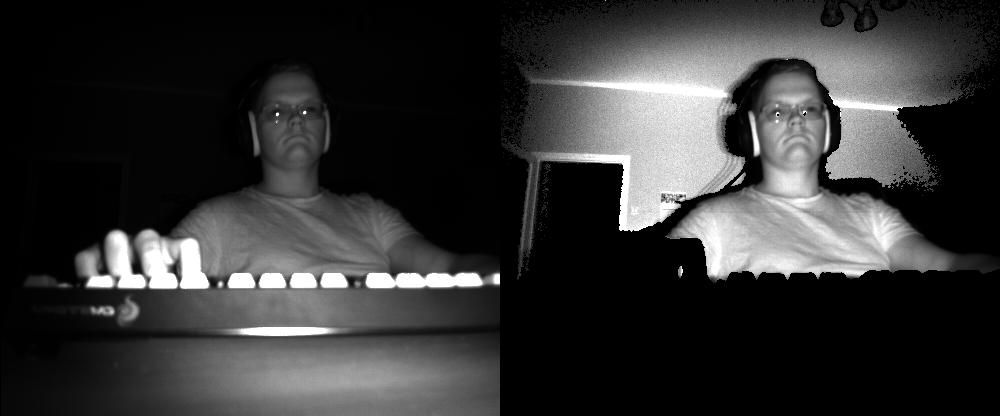
\includegraphics[width=\textwidth]{skin_kinect_1}
                \label{fig:skin_kinect_1}
            \end{figure}

            As seen on figure \ref{fig:skin_kinect_1}, we have accidentally created
            a night vision camera (please note that some of the black areas are there because Kinect cameras do not give depth data for objects closer than 50cm)
            -- but this means that our idea is to some extent working, because the point
            of it was to make objects in the distance indistinguishable from those close
            to the camera.

            However, one this that is not considered in that method is that objects
            can also be at different angles to the camera.
            A sheet of paper perpendicular to the source of light will reflect more
            light to the Kinect than it would reflect if it was at a 45 degrees angle.

            \begin{figure}[H]
                \caption{Three IR images processed with the described method, with a
                manually determined interval of values marked red.}
                \centering
                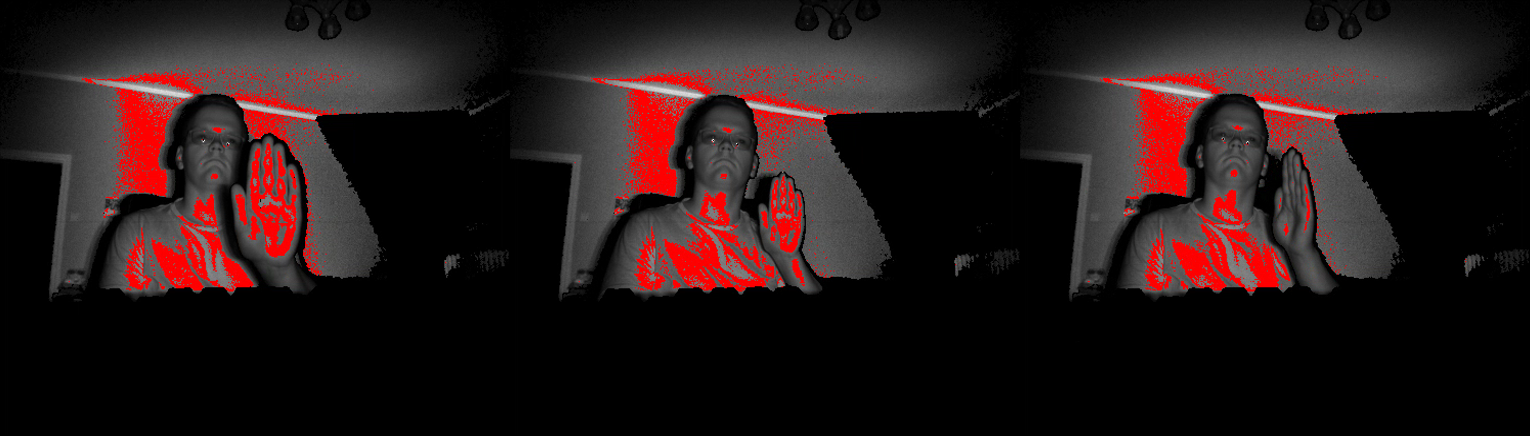
\includegraphics[width=\textwidth]{skin_kinect_2}
                \label{fig:skin_kinect_2}
            \end{figure}

            We have manually selected an interval of values and marked them red, which
            can be seen on figure \ref{fig:skin_kinect_2}.
            On the first two pictures there, the hand is at the same angle, but at a
            different distance to the camera.
            It is visible that the calculated values remained very close regardless
            of the distance, which was a success.
            However, on the third picture, the hand is at a different angle and
            that changes how it reflects light towards the camera, which makes the values
            different.

            Knowing the depth value and certain properties of the camera, it is possible
            to calculate the 3D coordinates of each pixel.
            With that information, it is possible to calculate the angle towards the
            camera between each two pixels, and then use that value in the method above
            to make it independent of angles.
            However, our attempts to do this were unsuccessful, possibly because the
            depth camera is not precise enough.
            % TODO Dominik: maybe describe briefly the mathematical details of what
            %               was attempted

        \subsubsection{Using three infrared wavelengths}

        TODO

    \subsection{Results}
        Wide discussion about results.

    \subsection{RGB skin detection symulation}
        Using RGB to deteckt skin on picture.
        Mtoivations.

        Description of not ours solutions.

        \subsubsection*{Case-study}
            Description of problem using math.
            Final algorithm.
